\vspace{-3mm}

\section{Background} 
\label{sec:back}





\textbf{Differential privacy \cite{dwork2014dpfoundations}.}  Formally, a randomized mechanism $\mathcal{M}$ is said to satisfy
$(\epsilon,\delta)$-differential privacy
if, for any two neighboring datasets $D$ and $D'$
that differ in exactly one data record,
and for any measurable subset $E$ of the output space,
the following condition holds:
$
\Pr[\mathcal{M}(D) \in E]
\leq e^{\epsilon} \Pr[\mathcal{M}(D') \in E] + \delta.
$ A common approach to achieving differential privacy in federated learning
is differentially private stochastic gradient descent (DP-SGD) \cite{abadi2016deep}.
Formally, let $g_i = \nabla_\theta \ell(\theta; x_i)$ denote the gradient
computed from a single training example $x_i$.
DP-SGD first applies per-sample gradient clipping. And the clipped gradients are then aggregated and perturbed with Gaussian noise:
$
\textit{(i)}\quad
g_i^{\mathrm{clip}} = g_i \cdot \min\!\left(1, \frac{C}{\|g_i\|_2}\right), \quad
\textit{(ii)}\quad
g^{\mathrm{noisy}} = \frac{1}{B}\left(\sum_{i=1}^{B} g_i^{\mathrm{clip}} + \mathcal{N}\!\left(0, \sigma^2 C^2 \mathbf{I}\right)\right),
$
where $C$ is a predefined clipping norm that bounds the sensitivity, $B$ is the batch size, $\sigma$ is the noise multiplier, and $\mathcal{N}(0, \sigma^2 C^2 \mathbf{I})$ denotes isotropic Gaussian noise.
Finally, the model parameters are updated using the noisy gradient:
$
\theta_{t+1} = \theta_t - \eta \, \bar{g},
$
where $\eta$ is the learning rate.
















\textbf{Aggregation error in federated LoRA \cite{wang2024flora}.} Given a pre-trained weight matrix $W_0 \in \mathbb{R}^{d_{out} \times d_{in}}$,
LoRA parameterizes the adapted weight as $W = W_0 + BA$, where $B \in \mathbb{R}^{d_{out} \times r}$ and $A \in \mathbb{R}^{r \times d_{in}}$.
In FL, the server aggregates local LoRAs $\{(A_k, B_k)\}_{k=1}^K$ via averaging as
$
\bar{A} = \frac{1}{K}\sum_{k=1}^K A_k, \quad
\bar{B} = \frac{1}{K}\sum_{k=1}^K B_k.
$
However, due to the multiplicative structure of LoRA,
$
\frac{1}{K}\sum_{k=1}^K B_k A_k \;\neq\; \bar{B}\,\bar{A}.
$
This mismatch leads to an aggregation error that accumulates across communication rounds,
and becomes more pronounced under heterogeneous client data distributions.


\begin{wrapfigure}{r}{0.36\linewidth}
    \centering
    \vspace{-5mm}
    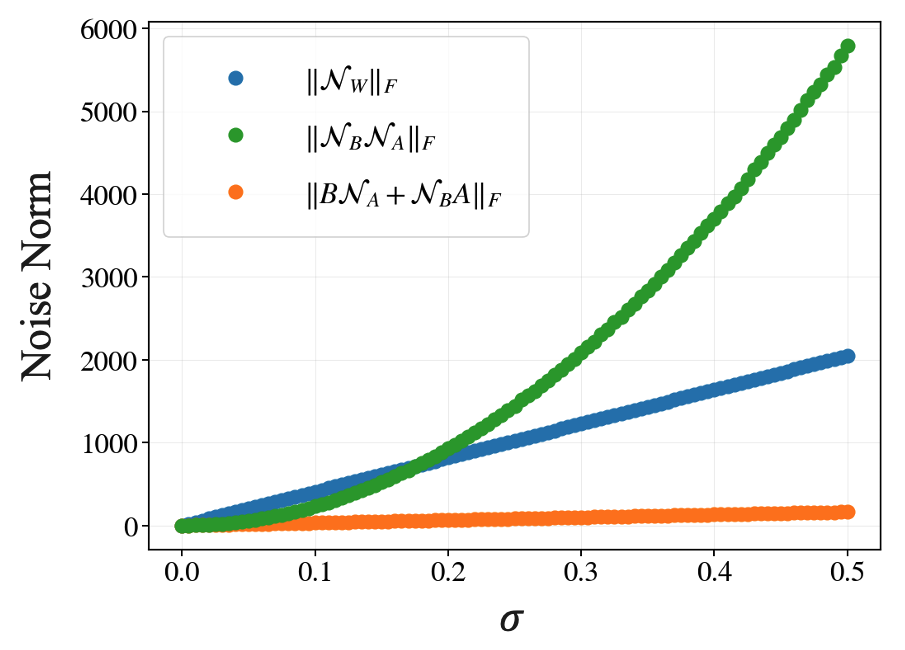
\includegraphics[width=\linewidth]{figures/3_background/noise_norm.png}
    \caption{
    Scaling behavior of different noise components with respect to the noise scale $\sigma$.
    }
    \label{fig:noise_norm}
    \vspace{-5mm}
\end{wrapfigure}

\textbf{DP noise amplification in LoRA \cite{sun2024improving}.} When DP-SGD is applied to LoRA parameters, Gaussian noise is added
to the gradients.
Let $\Delta B$ and $\Delta A$ denote the updates to $B$ and $A$ in a given round,
which consist of a true update component and a DP noise component:
$
\Delta B = \Delta B^{\star} + \mathcal{N}_B, \quad
\Delta A = \Delta A^{\star} + \mathcal{N}_A.
$
% where $\mathcal{N}_B$ and $\mathcal{N}_A$ are Gaussian noise terms
% induced by DP-SGD.
The resulting update to the effective weight matrix is given by
$\Delta W=B \Delta A^{\star}+\Delta B^{\star} A+B \mathcal{N}_A+\mathcal{N}_B A+\mathcal{N}_B \mathcal{N}_A$.
% $
% \Delta W=(B + \Delta B)(A + \Delta A) - BA.
% $
% Expanding this expression yields
% $
% \Delta W=B \Delta A+\Delta B A+\Delta B \Delta A.
% $
% Substituting the noisy updates, we obtain
% $
% \Delta W=B \Delta A^{\star}+\Delta B^{\star} A+\underbrace{B \mathcal{N}_A+\mathcal{N}_B A+\mathcal{N}_B \mathcal{N}_A}_{\text{DP-induced noise terms}}.
%$
As illustrated in Figure~\ref{fig:noise_norm}, different noise components exhibit distinct scaling behaviors with respect to the noise scale $\sigma$. 
The full-model noise $\|\mathcal{N}_W\|_F$ grows linearly, whereas the multiplicative cross-term $\|\mathcal{N}_B \mathcal{N}_A\|_F$ exhibits quadratic growth and becomes dominant as $\sigma$ increases. 
This phenomenon leads to \emph{noise amplification} in the effective model update, which can significantly degrade convergence and stability.

Additional related works are introduced in Appendix~\ref{sec:Appendix A}.

% \noindent\textbf{Notation.}
% We use $K$, $T$, and $N$ to denote the number of clients, communication rounds, and LoRA layers, and write the adapted weight at layer $n \in [N]$ and round $t$ as $W^t(n) = W_0(n) + B^t(n) A^t(n)$. The symbol $a \in \{A, B\}$ acts as a block selector that we use throughout the paper, and $g_a^{(n)} := \nabla_{a(n)} L$ and $H_a^{(n)} := \nabla_{a(n)}^2 L$ denote the stochastic gradient and population Hessian of the corresponding block at layer $n$. We write $N_a \sim \mathcal{N}(0, \sigma^2 C^2 I)$ for the DP-SGD noise injected into block $a$ under clipping bound $C$ and target $(\epsilon, \delta)$. Throughout, $\|\cdot\|_F$ denotes the Frobenius norm and $\|\cdot\|_2$ the spectral or Euclidean norm depending on its argument.